\chapter{Planung}

In diesem Kapitel werden Anforderungen an die Software und die Systemumgebung definiert sowie verwendete organisatorische Konzepte erläutert.

\section{Anforderungen}

Die Software soll auf den nicht-interaktiven Betrieb als Dienst auf unixoiden Betriebssystemen ausgelegt werden. Dies hat u.A. Auswirkungen auf die geplanten Benutzerschnittstellen. Das Programm soll zur Laufzeit keine Konsoleneingaben verlangen, da diese nur bei einem interaktiven Betrieb, z.B. in der Shell, vorgenommen werden können. Stattdessen soll mit dem Anwender vollständig über den Telegram-Messenger interagiert werden und administrative Einstellungen sollen über Konfigurationsdateien vorgenommen werden können. Zur Anwendung von geänderten Einstellungen ist u.U. ein Neustart der Software notwendig. Die Software sollte daher zustandslos arbeiten, um einen möglichen Verlust von eingegangenen und noch nicht verarbeiteten Daten zu verhindern. Weiterhin sollte die durch einen Neustart verursachte Ausfallzeit so gering wie möglich gehalten werden. Die Software soll Ereignismeldungen über die Standardausgabe sowie über eine textbasierte Protokolldatei ausgeben, um Fehleranalysen zu vereinfachen. Es soll möglich sein, den Bot von mehreren Geräten gleichzeitig zu kontaktieren. Der Bot muss die Autorisierung von Benutzern prüfen, damit unerwünschter Datenabfluss verhindert wird.

\subsection{Systemkonfiguration}
Für den Betrieb der Software ist eine vorinstallierte Python 3 Umgebung notwendig. Zum Zeitpunkt der Entwicklung wurde die Version 3.9 verwendet. Die benötigten Bibliotheken sollen über den Paketmanager pip bezogen und aktuell gehalten werden können. Auch wenn die Software auf den Betrieb als Dienst ausgelegt werden soll, soll eine interaktive Verwendung sowohl mit unixoiden Betriebssystemen als auch mit Windows möglich sein. Außerdem ist eine Internetverbindung notwendig, um die HTTP-APIs von Telegram und AWS zu erreichen. Graylog Open muss bereits installiert und an die zu überwachende Systeme angeschlossen sein. Die Systemanforderungen entsprechen denen des verwendeten Betriebssystems.

\section{Programmablauf}

\subsection{Grundsätzlicher Aufbau}
\label{sec:grundsaetzlicher-aufbau}

Nach dem Start der Software muss geprüft werden, ob ein einwandfreier Betrieb möglich ist. Dazu ist es notwendig, die Erreichbarkeit und Funktion sämtlicher Dienste mittels geeigneter API-Abfragen zu prüfen. Nachdem die Vorbereitungen abgeschlossen sind, kann in den Regelbetrieb übergegangen werden, in welchem sich das Programm bis zum Programmende befindet. 

\subsection{Regelbetrieb}

Im Regelbetrieb reagiert die Software in Echtzeit auf eingehende Nachrichten vom Anwender. 
Um den Betrieb der Software auch mit nicht-öffentlichen IP-Adressen (beispielsweise in einem Heimnetzwerk hinter einem NAT-Router oder einer Firewall) zu ermöglichen, soll das Verfahren des 'long-polling' für den Abruf von Informationen von der Telegram API verwendet werden (vgl. \autoref{sec:telegram-getting-updates}).

Der geplante Ablauf des Regelbetriebs ist in folgendem Sequenzdiagramm abgebildet:

\newpage

\begin{figure}[h!]
\centering
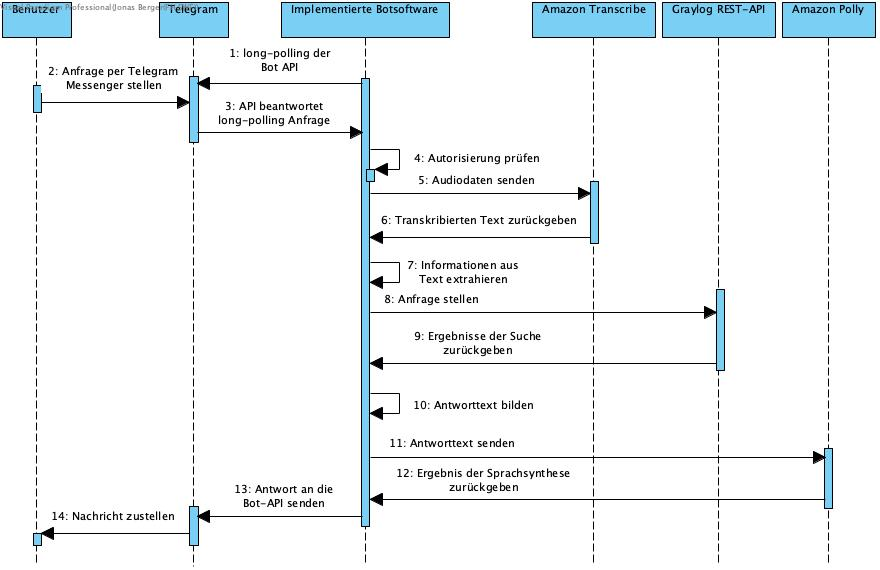
\includegraphics[scale=0.7]{dia-seq}
\caption{Sequenzdiagramm für Regelbetrieb.}
\end{figure}

\subsection{Spracherkennung}

Bei der Ausarbeitung eines Konzepts für die Funktionsweise der Spracherkennung müssen einige funktionale und nicht-funktionale Eigenschaften beachtet werden. Die Entscheidung wird u.A. beeinflusst durch Aspekte der... 

\begin{itemize}
\item Erweiterbarkeit: es soll einfach und insbesondere ohne ein notwendiges Training von Sprachmodellen möglich sein, neue Systeme und Abfragen zu definieren.
\item Fehlertoleranz: gesprochene Sprache enthält Umgangssprache und verändert sich durch grammatikalische Eigenschaften je nach Satzbau leicht in der Aussprache. Die Erkennung muss trotz dieser Veränderungen zuverlässig funktionieren.
\item Rechenkapazität: die Geschwindigkeit (Wartezeit während dem Vorgang) der Spracherkennung sollte nicht von limitierten Rechenressourcen oder der Länge der zu übersetzenden Sprache abhängen.
\item finanziellen Kosten: diese sollten möglichst gering gehalten werden.
\item Plattformunabhängigkeit: die Software und ggf. trainierte Modelle sollten wie die gewählte Programmiersprache Python plattformunabhängig und portabel sein.
\item Nachvollziehbarkeit: während der Entwicklung und bei der Definition neuer Begriffe sollten auftretende Fehler einfach erkenn- und behebbar sein.
\item Sprache: das System soll Sätze verstehen, welche Begriffe aus mehreren Sprachen (deutsch und englisch) beinhalten.
\end{itemize}

Es bestehen verschiedene Möglichkeiten, Sprache zu Text zu transkribieren und den Inhalt im Anschluss zu analysieren, um das Anliegen des Anwenders zu erkennen und eine passende Anfrage für die Suchmaschine in Graylog zu bilden. Für die Transkription ist es notwendig, künstliche Intelligenz einzusetzen. Diese kann lokal oder entfernt ausgeführt werden. Die entfernte Ausführung bietet Vorteile bezüglich der Plattformunabhängigkeit und der (von den lokalen Ressourcen unabhängigen) Geschwindigkeit. Es stehen verschiedene gleichwertige Online-Dienste für die Transkription zur Verfügung, darunter 'Watson Speech to Text' von IBM und 'Amazon Transcribe' von AWS.

\subsubsection{Syntax}
\label{sec:syntax}

Liegt die eingegangene Nachricht als Text vor, müssen die Inhalte analysiert werden. Aufgrund des notwendigen Trainings für neue Begriffsdefinitionen ist der Einsatz von künstlicher Intelligenz bei dieser Programmkomponente nicht sinnvoll. Der Aufbau der Nachricht muss stattdessen einem festen Muster folgen, welches durch eine Prozedur analysiert werden kann. Hierzu eignet sich die Verwendung von Schlüsselwörtern. Diese bieten den Vorteil, dass keine Analyse der Grammatik notwendig ist. Um die Erweiterung zu vereinfachen, wird ein Aufbau aus Produktkategorie, Eigenschaft und Zeitraum gewählt. Die Produktkategorie entspricht der abzufragenden Gerätegruppe, beispielsweise \lstinline{Webserver}. Für jede Produktkategorie können Eigenschaften definiert werden, für die Abfrage von Ereignissen mit einem Statuscode \lstinline{4xx} oder \lstinline{5xx} der Gruppe \lstinline{Webserver} beispielsweise \lstinline{Fehlermeldungen}. Ein weiteres Schlüsselwort führt zu den Informationen für den abzufragenden Zeitraum, welcher relativ angegeben wird (\lstinline{letzte fünf Tage}, \lstinline{letzte Woche}, \lstinline{letzte 20 Minuten}). Schließlich muss die Erkennung von Zahlwörtern zuverlässig funktionieren.

\subsubsection{Verknüpfung geeigneter Suchbegriffe}

Die Erweiterung der Software soll einfach möglich sein. Produktgruppen sollten darüber hinaus dynamisch erweiterbar sein: wird eine Abfrage für die Produktkategorie \lstinline{Webserver} getätigt, sollen alle derzeit an Graylog angeschlossenen Webserver in die Suche einbezogen werden. Die Software ist für die Bedienung von Systemadministratoren vorgesehen. Daher soll für die Konfiguration der Abfragen eine Textdatei verwendet werden. Diese ermöglicht eine schnelle Anpassung der Konfiguration und bietet gleichzeitig einen Überblick über bestehende Suchbegriffe. Für die einfache Verwendung mit einer Bibliothek Python stehen mehrere Dateiformate zur Verfügung, darunter JSON, INI, TOML, YAML und XML. Das YAML- und XML-Format ist für die Verwaltung über einen Texteditor ohne Syntaxhervorhebung und Funktionen wie automatischem Einrücken nicht geeignet. Das TOML-Format vereint die Vorteile der einfachen Lesbarkeit des INI-Formats mit der Fehlerunanfälligkeit bei der Verarbeitung durch Maschinen des JSON-Formats. TOML entspricht weitestgehend der INI-Syntax mit dem Unterschied, dass Anführungszeichen verwendet werden können, um Anfang und Ende von Werten zu markieren. Die Hierarchie innerhalb einer TOML-Datei stimmt mit dem in \autoref{sec:syntax} gebildeten Aufbau überein. Sektionen werden mit eckigen Klammern markiert und entsprechen den Produktkategorien. Sie beinhalten Name-Wert-Paare, welche durch ein Gleichheitszeichen getrennt werden. Ein Name darf in einer Sektion nur jeweils einmal vorkommen, eine Sektion darf in einer Datei nur jeweils einmal vorkommen. Bestehen Namen aus mehreren Wörtern, können diese mit Anführungszeichen zusammengefasst werden. Namen entsprechen den oben definierten Eigenschaften von Produktkategorien. Werte entsprechen grundsätzlich einem festgelegten Datentyp. Strings (Zeichenketten) werden in Anführungszeichen geschrieben. Die Werte einer TOML-Datei entsprechen den mit Eigenschaften verknüpften Suchbegriffen. Zusätzlich ist es möglich, einzeilige Kommentare mit \lstinline{#} einzuleiten.

\begin{lstlisting}[caption={Beispiel der TOML-Syntax.}, label=toml-syntax]
# Dies ist ein Kommentar
[Sektion]
Name = "Wert"

[Webserver]
Fehler = http_response_code:[400 TO 599] 
\end{lstlisting}
